\section{Contextual Bandits}
\label{sec:bandits_results}

\subsection{Design}
\label{sec:bandits_design}

This experiment preserves the affiliated valuation model from Experiment~1b but replaces Q-learning with contextual bandit methods. Table~\ref{tab:exp2_params} summarises the parameters. Seven binary factors and the three-level affiliation parameter $\eta$ define the experimental space. LinUCB includes two additional factors (regularisation $\lambda$ and memory decay) that preliminary screening found negligible for Thompson Sampling. These are excluded from the Thompson Sampling design to concentrate cells on active factors.\footnote{The exploration intensity factor maps to algorithm-specific parameters. For LinUCB, the confidence bound width $c \in \{0.5, 2.0\}$ (a 4$\times$ ratio), and for Contextual Thompson Sampling, the posterior variance $\sigma^2 \in \{0.1, 1.0\}$ (a 10$\times$ ratio). These ratios reflect the different units and scales of the two exploration mechanisms. LinUCB explores by inflating the estimated reward with $c\sqrt{\mathbf{x}^\top A^{-1}\mathbf{x}}$, where the uncertainty term shrinks with data; a 4$\times$ increase in $c$ roughly quadruples the exploration bonus. Thompson Sampling explores through posterior sampling variance $\sigma^2 A^{-1}$; a 10$\times$ increase broadens the sampling distribution proportionally. The factorial model captures this asymmetry through the algorithm $\times$ exploration intensity interaction term.}\footnote{The memory decay factor $\delta$ controls how much weight historical observations receive relative to recent ones. At $\delta = 1.0$ (no decay), both LinUCB and Thompson Sampling accumulate all past data, and after $T$ rounds the effective sample size is $T$. At $\delta < 1$, the effective sample size plateaus at approximately $1/(1-\delta)$. This factor is motivated by \citet{Douglas2024}, who show that deterministic convergence in bandit learners drives collusive outcomes, and by \citet{Russac2019}, who provide regret guarantees for discounted linear bandits in non-stationary environments.}

\begin{table}[H]
\centering
\caption{Parameter settings for Experiments~2a and~2b (Affiliated Valuations + Bandits).}
\label{tab:exp2_params}
\begin{tabular}{l l l}
\toprule
\textbf{Factor} & \textbf{Low ($-1$)} & \textbf{High ($+1$)}\\
\midrule
Algorithm & LinUCB & CTS \\
Auction format & Second-price & First-price \\
Number of bidders ($n$) & 2 & 4 \\
Reserve price ($r$) & 0.0 & 0.3 \\
Exploration intensity & Low & High \\
Context richness & Signal only & Signal + winner \\
Regularisation ($\lambda$) & 0.1 & 5.0 \\
Memory decay ($\delta$) & 1.0 (no decay) & 0.999 (active) \\
\midrule
\textbf{Factor} & \multicolumn{2}{l}{\textbf{Levels}} \\
\midrule
Affiliation ($\eta$) & \multicolumn{2}{l}{0, 0.5, 1 (linear + quadratic contrasts)} \\
\midrule
\multicolumn{3}{l}{\textbf{Fixed parameters}} \\
\midrule
Bid grid resolution & \multicolumn{2}{l}{11 discrete actions} \\
Number of rounds & \multicolumn{2}{l}{100{,}000} \\
\bottomrule
\end{tabular}
\end{table}

\subsection{LinUCB (Experiment~2a)}
\label{sec:exp2a_results}

Experiment~2a deploys LinUCB agents under the affiliated valuation model. The design is a $3 \times 2^7 = 384$ mixed-level factorial with 8 factors (7 binary plus the three-level affiliation parameter $\eta$), including the regularisation parameter $\lambda$ and memory decay, both of which strongly affect LinUCB performance. The design is replicated twice for \ExpTwoANobs{} observations.

\begin{figure}[H]
  \centering
  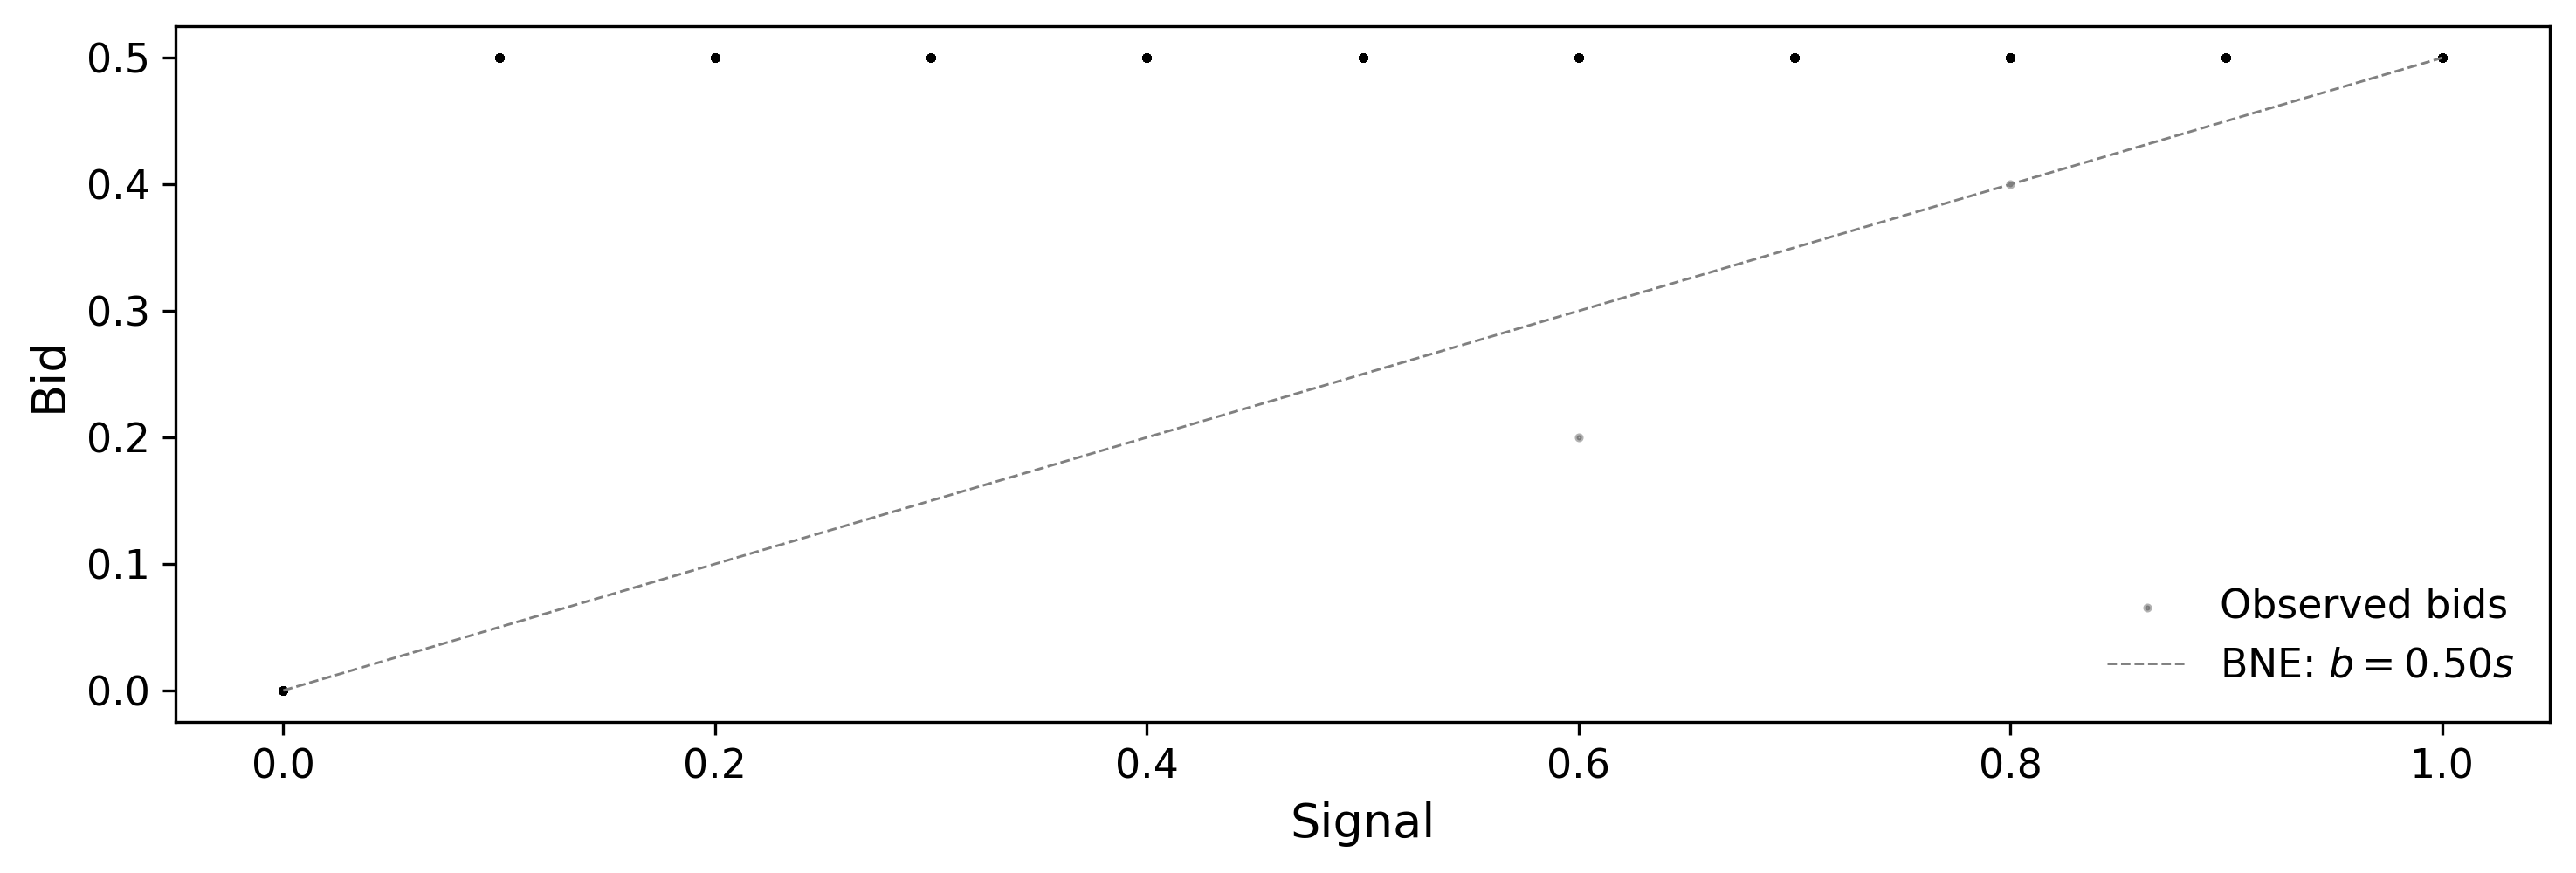
\includegraphics[width=\textwidth]{figures/e2a_trace}
  \caption{Representative bid function for a single trial of Experiment~2a (LinUCB, first-price auction, $\eta = 0.5$, 2~bidders, 5{,}000 rounds). Bids versus signals in the final 1{,}000 rounds, overlaid with the BNE bid function.}
  \label{fig:e2a_trace}
\end{figure}

\subsubsection{Revenue}

Number of bidders dominates ($|t| = \ExpTwoARevFactorTOne$), with the shift from two to four bidders increasing revenue by \ExpTwoARevTopPctEffect\% of the grand mean. The next largest effects are \ExpTwoARevFactorTwo{} ($|t| = \ExpTwoARevFactorTTwo$) and \ExpTwoARevFactorThree{} ($|t| = \ExpTwoARevFactorTThree$). Table~\ref{tab:exp2a_ranked_rev} ranks all significant effects by absolute $t$-statistic. First-price auctions yield lower final revenue ($|t| = \ExpTwoARevAuctionT$), as the main effects plot (Figure~\ref{fig:e2a_main_rev}) confirms.

\begin{table}[H]
\centering
\caption{Experiment 2a: Significant effects for average revenue ($p < 0.05$), ranked by $|t|$.}
\label{tab:exp2a_ranked_rev}
\begin{tabular}{lrrl}
\toprule
\textbf{Effect} & \textbf{Coeff.} & \textbf{$|t|$} & \textbf{Direction} \\
\midrule
Number of bidders & 0.1308 & 33.90 & + \\
Auction format & -0.0482 & 12.49 & $-$ \\
Number of bidders $\times$ Reserve price & -0.0400 & 10.36 & $-$ \\
Auction format $\times$ Number of bidders & -0.0245 & 6.35 & $-$ \\
Reserve price $\times$ Context richness & -0.0223 & 5.78 & $-$ \\
Affiliation (linear) & -0.0135 & 5.71 & $-$ \\
Affiliation (linear) $\times$ Affiliation (quadratic) & -0.0135 & 5.71 & $-$ \\
Exploration intensity & -0.0168 & 4.37 & $-$ \\
Auction format $\times$ Reserve price & 0.0150 & 3.88 & + \\
Exploration intensity $\times$ Context richness & 0.0137 & 3.54 & + \\
\bottomrule
\end{tabular}
\end{table}


\begin{figure}[H]
  \centering
  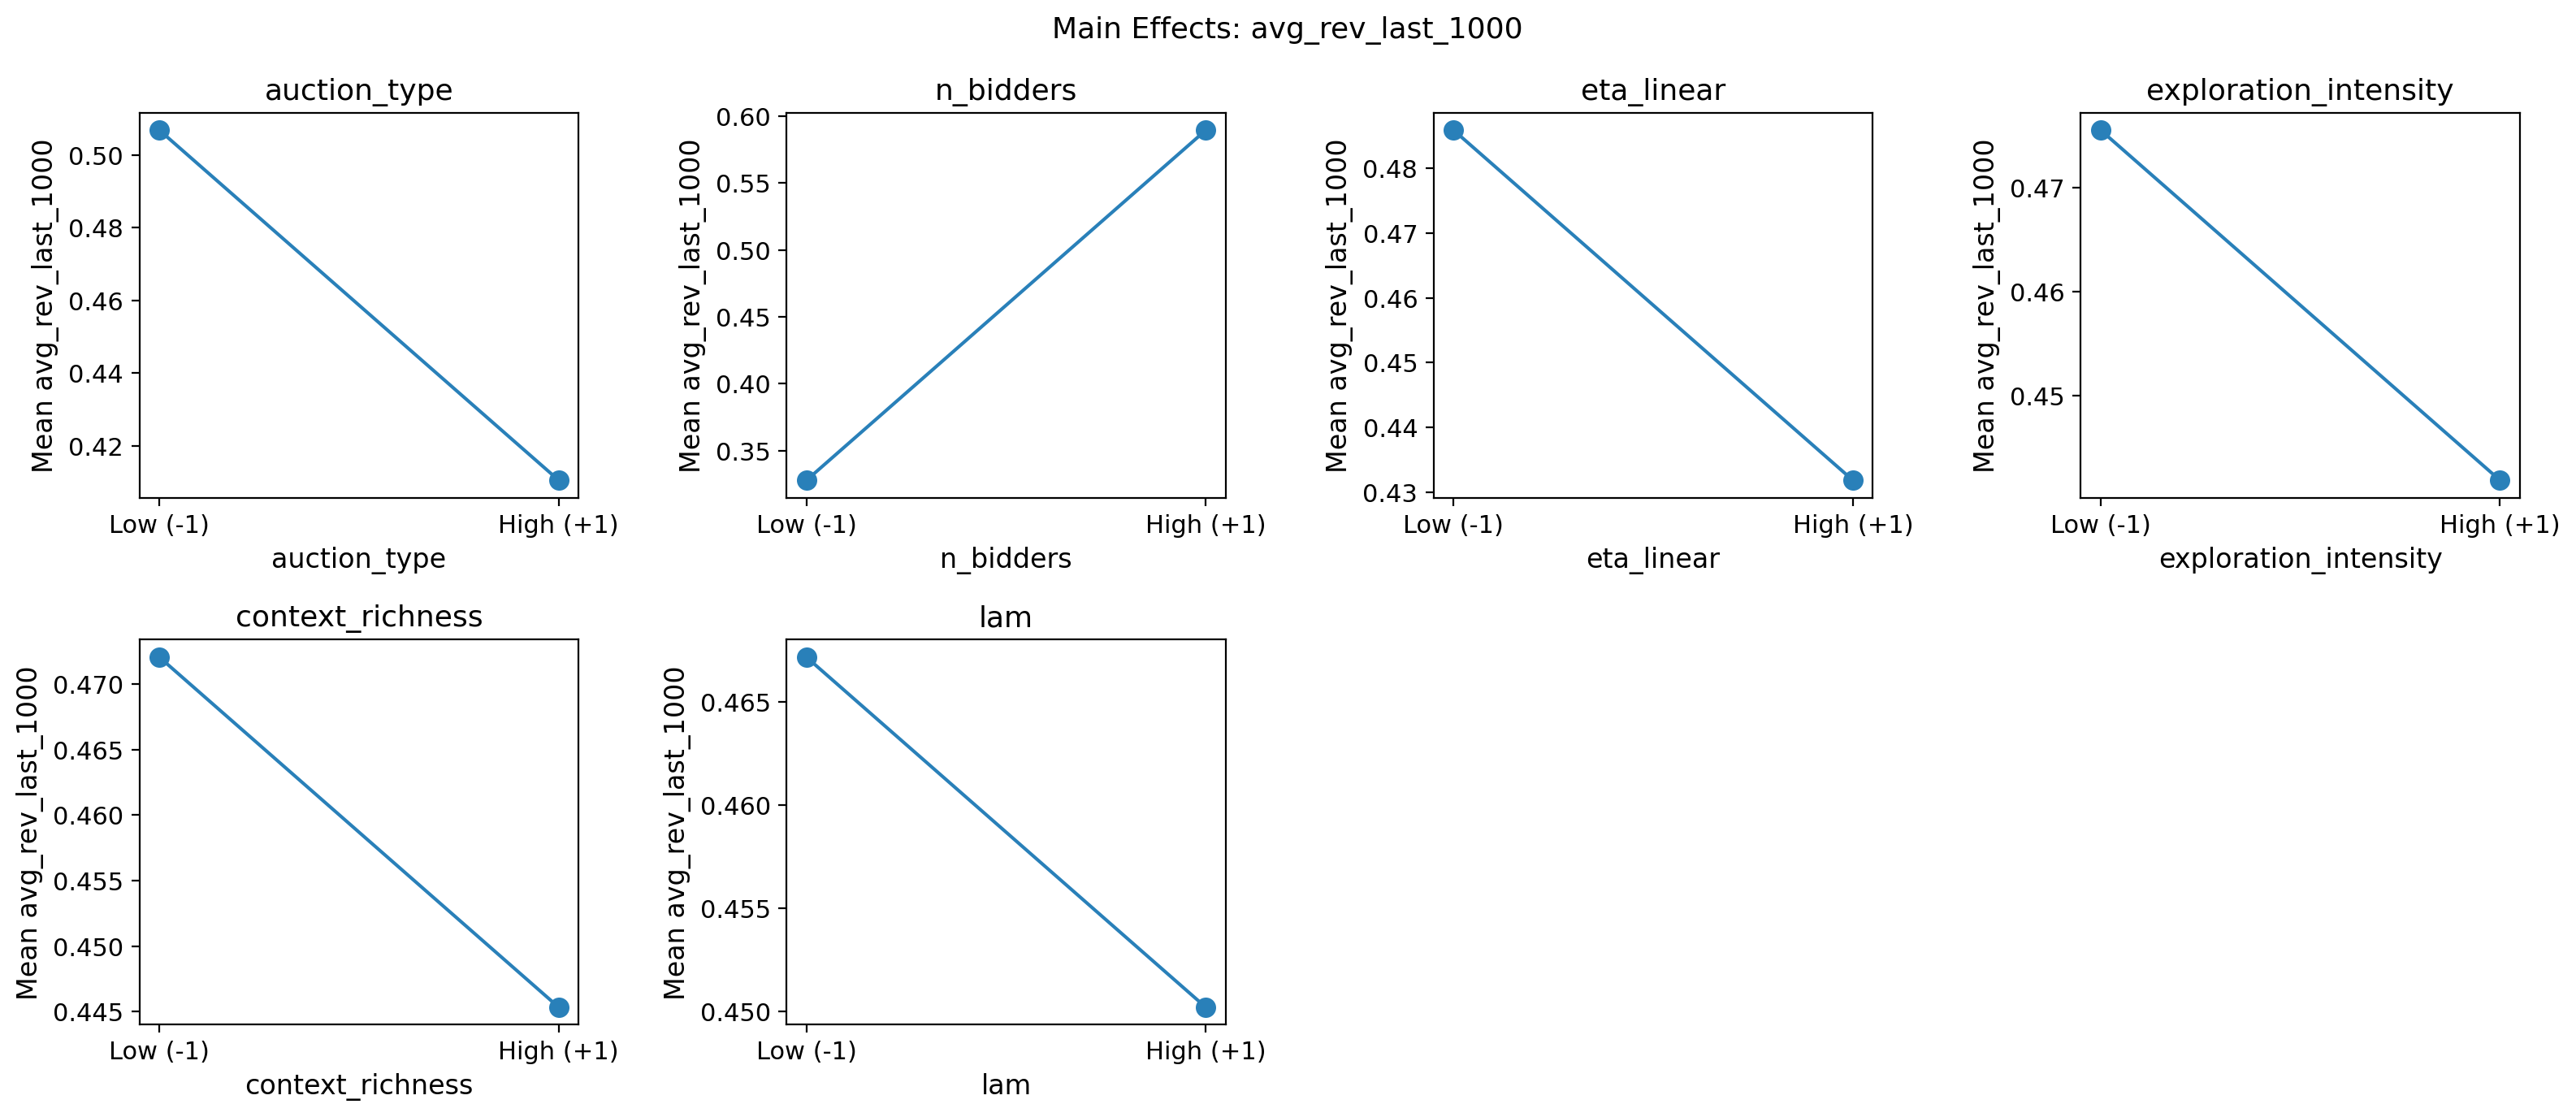
\includegraphics[width=0.7\textwidth]{figures/e2a_main_rev}
  \caption{Experiment~2a: Main effects plot for average revenue under LinUCB.}
  \label{fig:e2a_main_rev}
\end{figure}

The top interaction effects appear in Figure~\ref{fig:e2a_int_rev}.

\begin{figure}[H]
  \centering
  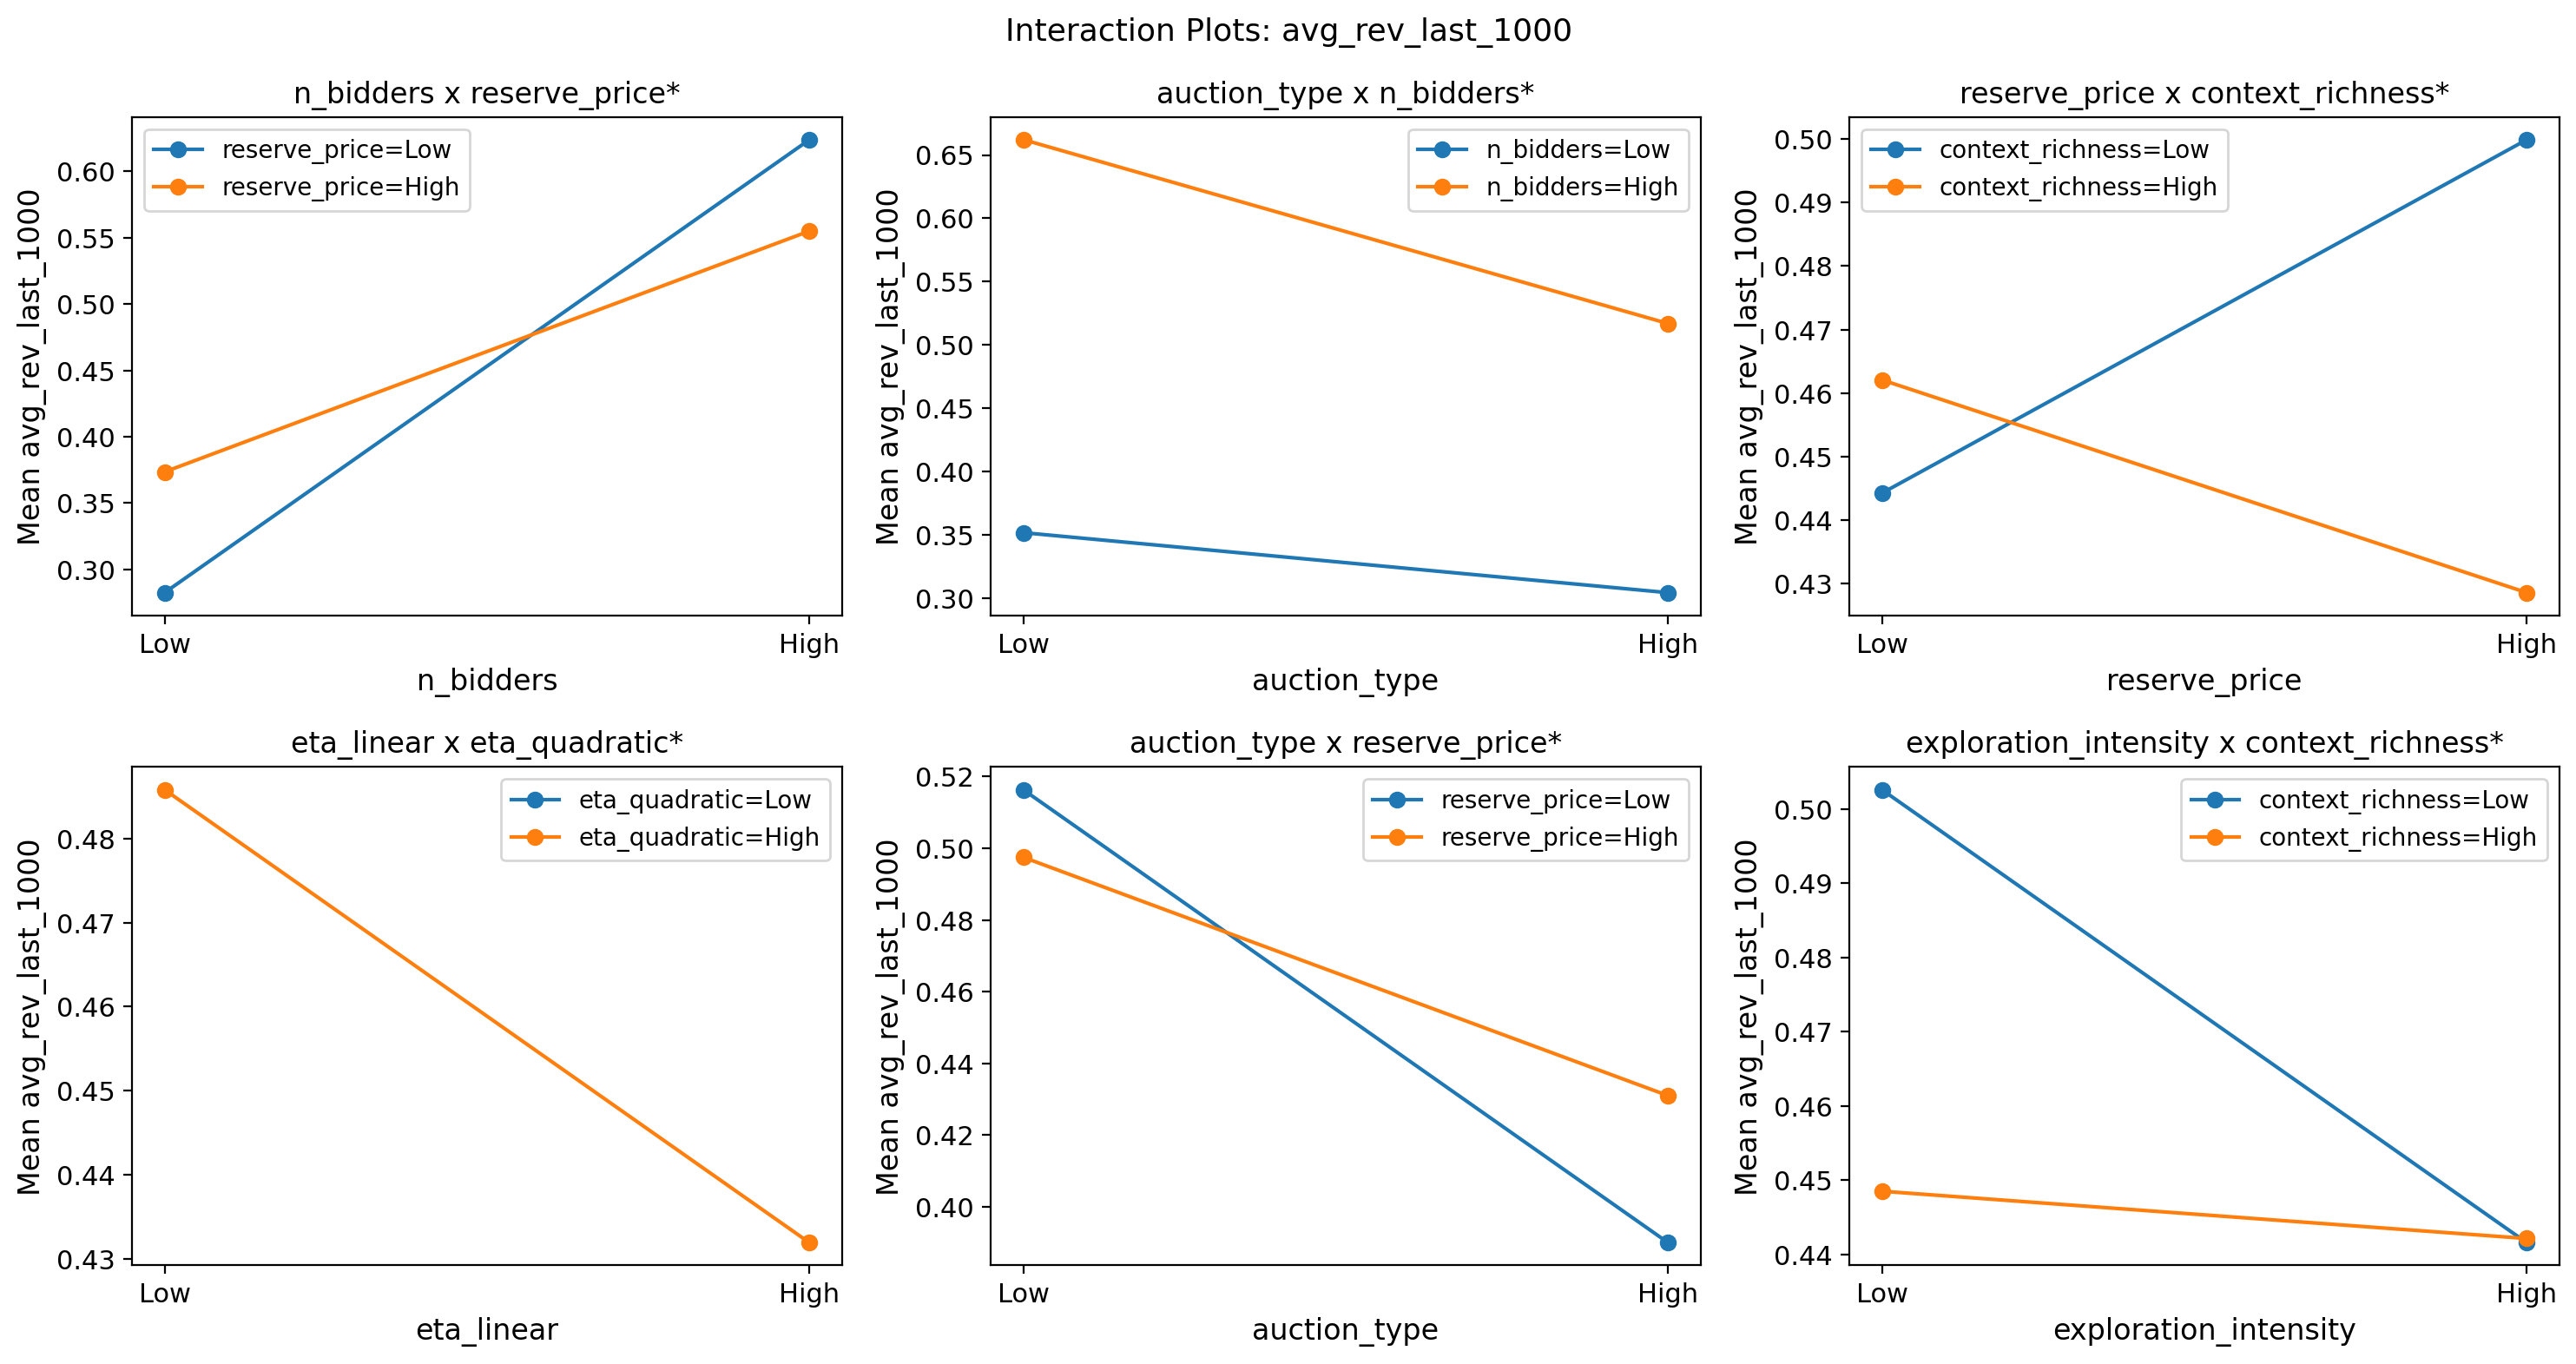
\includegraphics[width=0.7\textwidth]{figures/e2a_int_rev}
  \caption{Experiment~2a: Interaction plot for average revenue under LinUCB. Non-parallel lines indicate factor interdependencies.}
  \label{fig:e2a_int_rev}
\end{figure}

\subsubsection{Price Volatility}

Table~\ref{tab:exp2a_ranked_vol} and the main effects plot (Figure~\ref{fig:e2a_main_vol}) show the factor rankings for price volatility under LinUCB.

\begin{table}[H]
\centering
\caption{Experiment 2a: Significant effects for price volatility ($p < 0.05$), ranked by $|t|$.}
\label{tab:exp2a_ranked_vol}
\begin{tabular}{lrrl}
\toprule
\textbf{Effect} & \textbf{Coeff.} & \textbf{$|t|$} & \textbf{Direction} \\
\midrule
Context richness & 0.0246 & 16.91 & + \\
Auction format $\times$ Number of bidders & 0.0227 & 15.61 & + \\
Auction format & -0.0194 & 13.38 & $-$ \\
Number of bidders & -0.0179 & 12.31 & $-$ \\
Regularisation ($\lambda$) & -0.0109 & 7.48 & $-$ \\
Number of bidders $\times$ Reserve price & 0.0100 & 6.91 & + \\
Exploration intensity & 0.0098 & 6.75 & + \\
Memory decay ($\gamma_m$) & -0.0077 & 5.29 & $-$ \\
Auction format $\times$ Reserve price & -0.0070 & 4.81 & $-$ \\
Affiliation (linear) $\times$ Affiliation (quadratic) & -0.0040 & 4.53 & $-$ \\
\bottomrule
\end{tabular}
\end{table}


\begin{figure}[H]
  \centering
  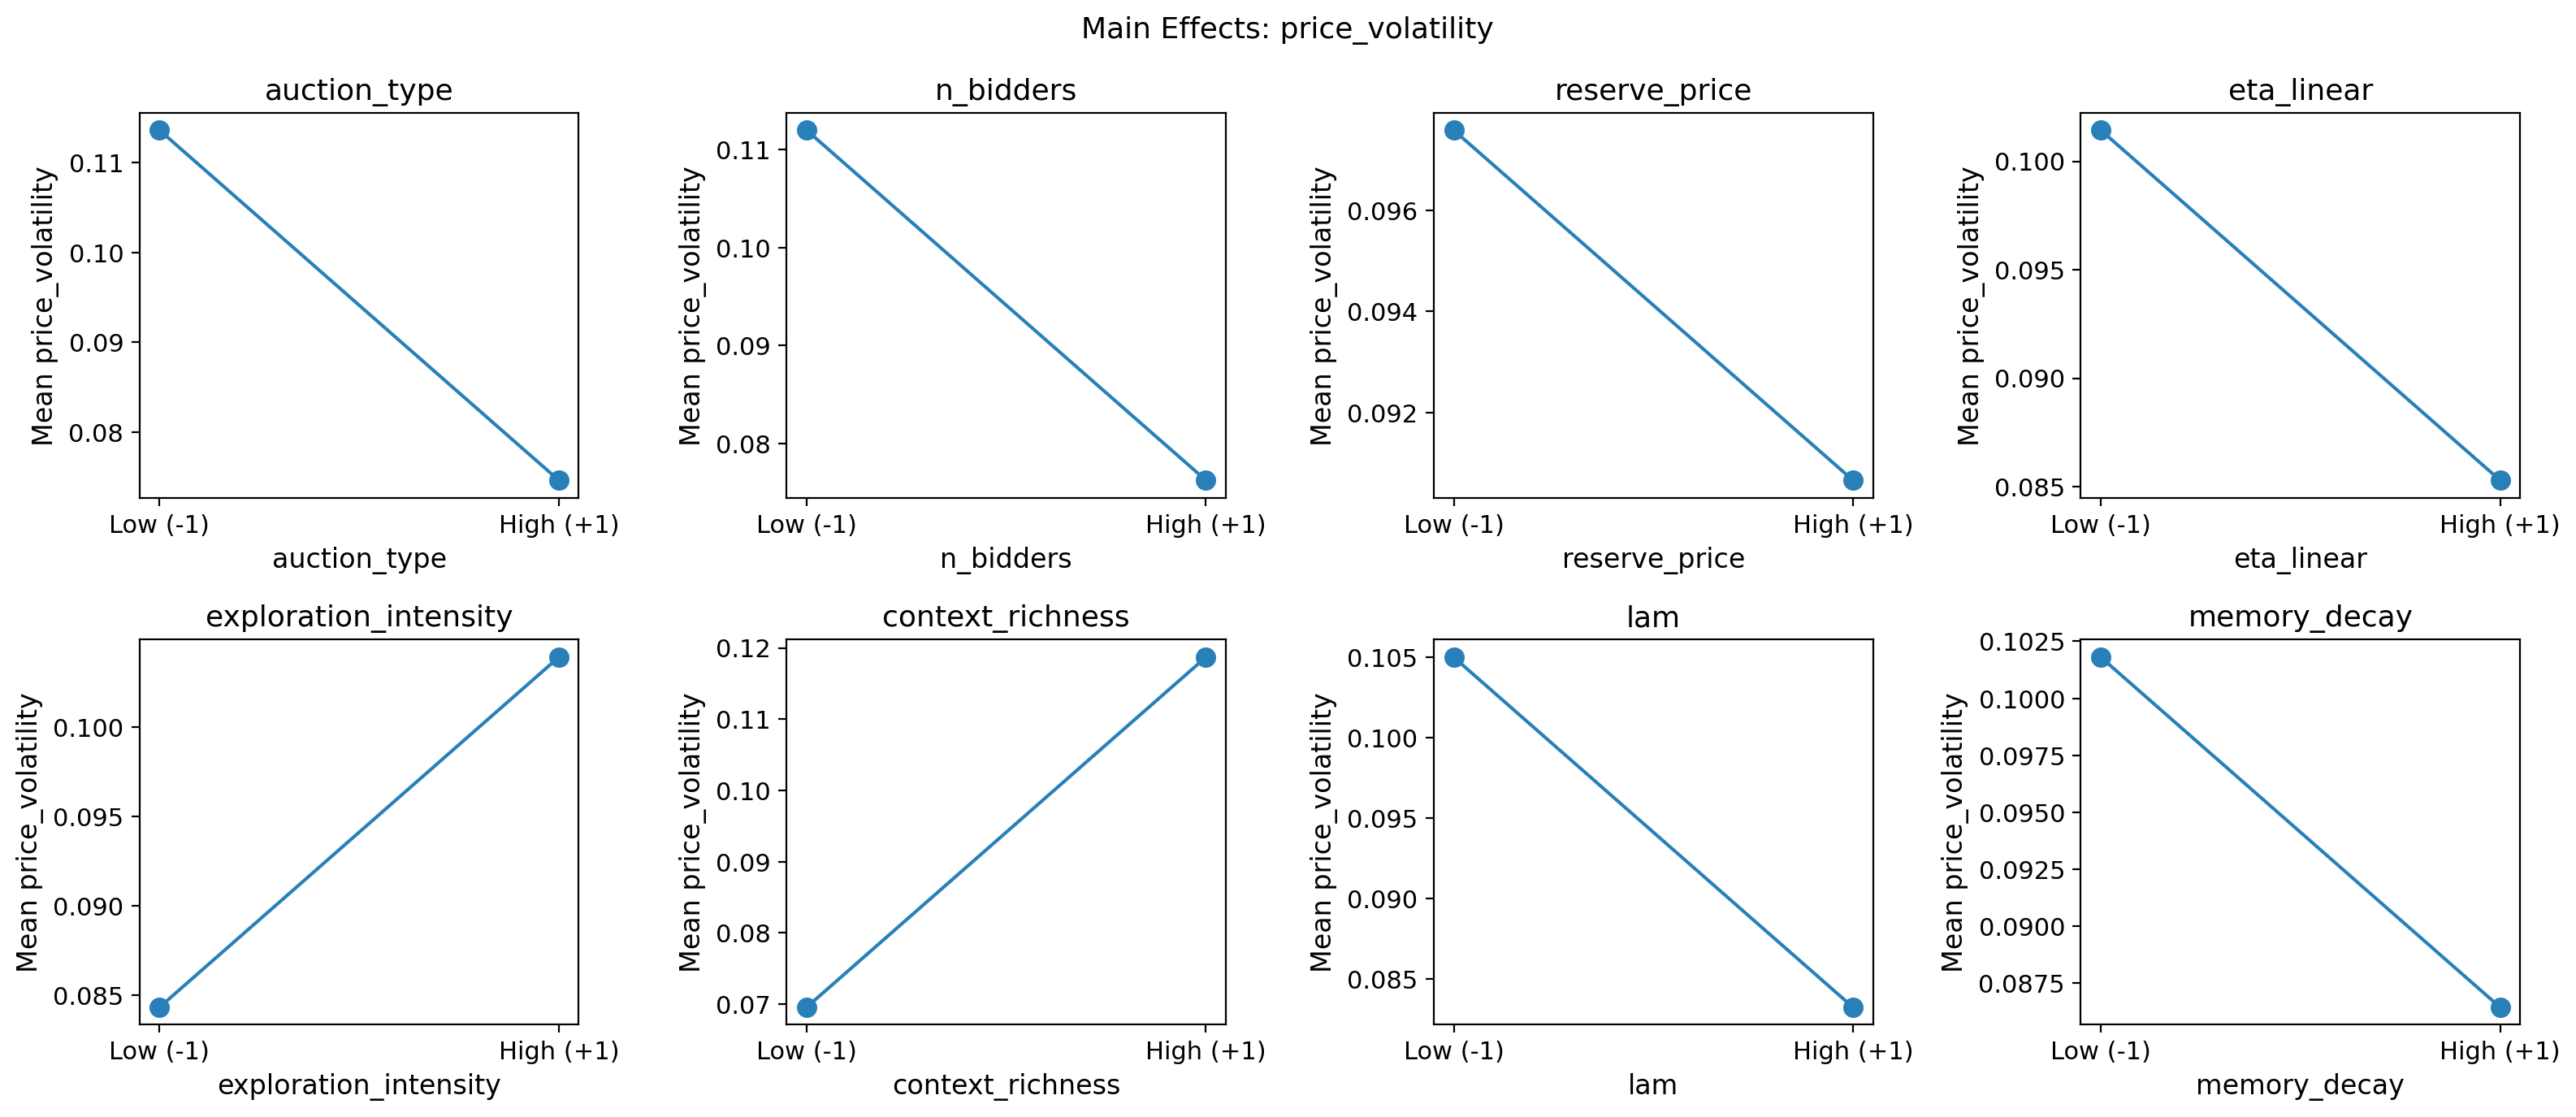
\includegraphics[width=0.7\textwidth]{figures/e2a_main_vol}
  \caption{Experiment~2a: Main effects plot for price volatility under LinUCB.}
  \label{fig:e2a_main_vol}
\end{figure}

Model adequacy diagnostics confirm these findings (Appendix~\ref{sec:appendix_robustness}).

\subsection{Contextual Thompson Sampling (Experiment~2b)}

Experiment~2b deploys Contextual Thompson Sampling agents under the same affiliated valuation model. The design is a $3 \times 2^5 = 96$ mixed-level factorial with 6 factors (5 binary plus $\eta$). Preliminary screening confirmed that $\lambda$ and memory decay have no detectable effect on Thompson Sampling outcomes, so both are excluded to avoid allocating design cells to factors with no detectable effect. The design is replicated twice for \ExpTwoBNobs{} observations.

\begin{figure}[H]
  \centering
  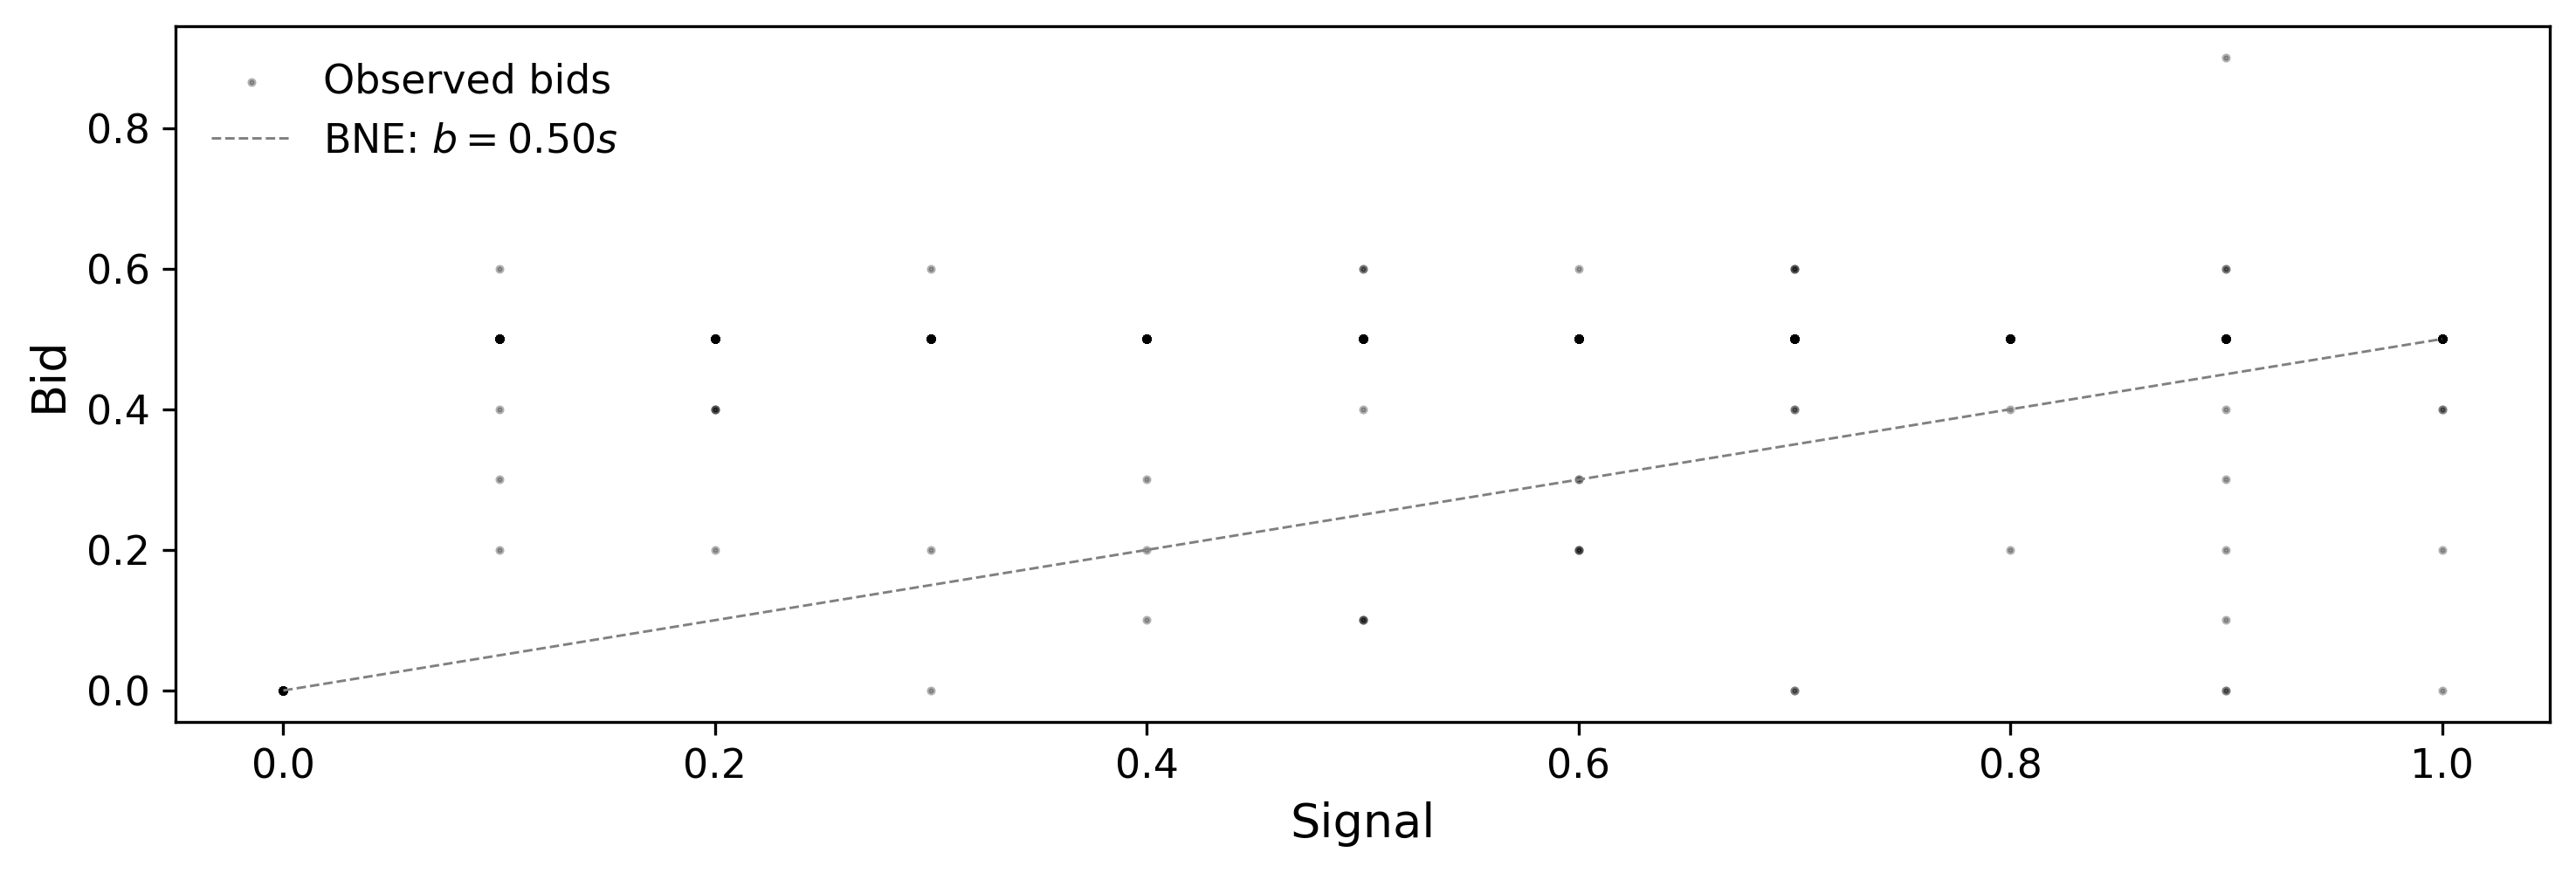
\includegraphics[width=\textwidth]{figures/e2b_trace}
  \caption{Representative bid function for a single trial of Experiment~2b (Thompson Sampling, first-price auction, $\eta = 0.5$, 2~bidders, 5{,}000 rounds).}
  \label{fig:e2b_trace}
\end{figure}

\subsubsection{Revenue}

Under Thompson Sampling, \ExpTwoBRevFactorOne{} dominates ($|t| = \ExpTwoBRevFactorTOne$), with the effect amounting to \ExpTwoBRevTopPctEffect\% of the grand mean, followed by \ExpTwoBRevFactorTwo{} ($|t| = \ExpTwoBRevFactorTTwo$). Table~\ref{tab:exp2b_ranked_rev} ranks all significant effects.

\begin{table}[H]
\centering
\caption[Experiment 2b: significant effects for average revenue ($p < 0.05$), ranked by $|t|$]{\textbf{Experiment 2b: significant effects for average revenue ($p < 0.05$), ranked by $|t|$.}}
\label{tab:exp2b_ranked_rev}
\begin{tabular}{lrrl}
\toprule
\textbf{Effect} & \textbf{Coeff.} & \textbf{$|t|$} & \textbf{Direction} \\
\midrule
Number of bidders & 0.0525 & 8.69 & + \\
Reserve price & -0.0480 & 7.95 & $-$ \\
Number of bidders $\times$ Context richness & 0.0284 & 4.71 & + \\
Auction format $\times$ Number of bidders & -0.0245 & 4.07 & $-$ \\
Auction format & -0.0231 & 3.83 & $-$ \\
Exploration intensity & -0.0204 & 3.38 & $-$ \\
Affiliation (linear) $\times$ Affiliation (quadratic) & -0.0117 & 3.18 & $-$ \\
Affiliation (linear) & -0.0117 & 3.18 & $-$ \\
Context richness & -0.0175 & 2.89 & $-$ \\
Number of bidders $\times$ Reserve price & -0.0174 & 2.88 & $-$ \\
\bottomrule
\end{tabular}
\end{table}


\begin{figure}[H]
  \centering
  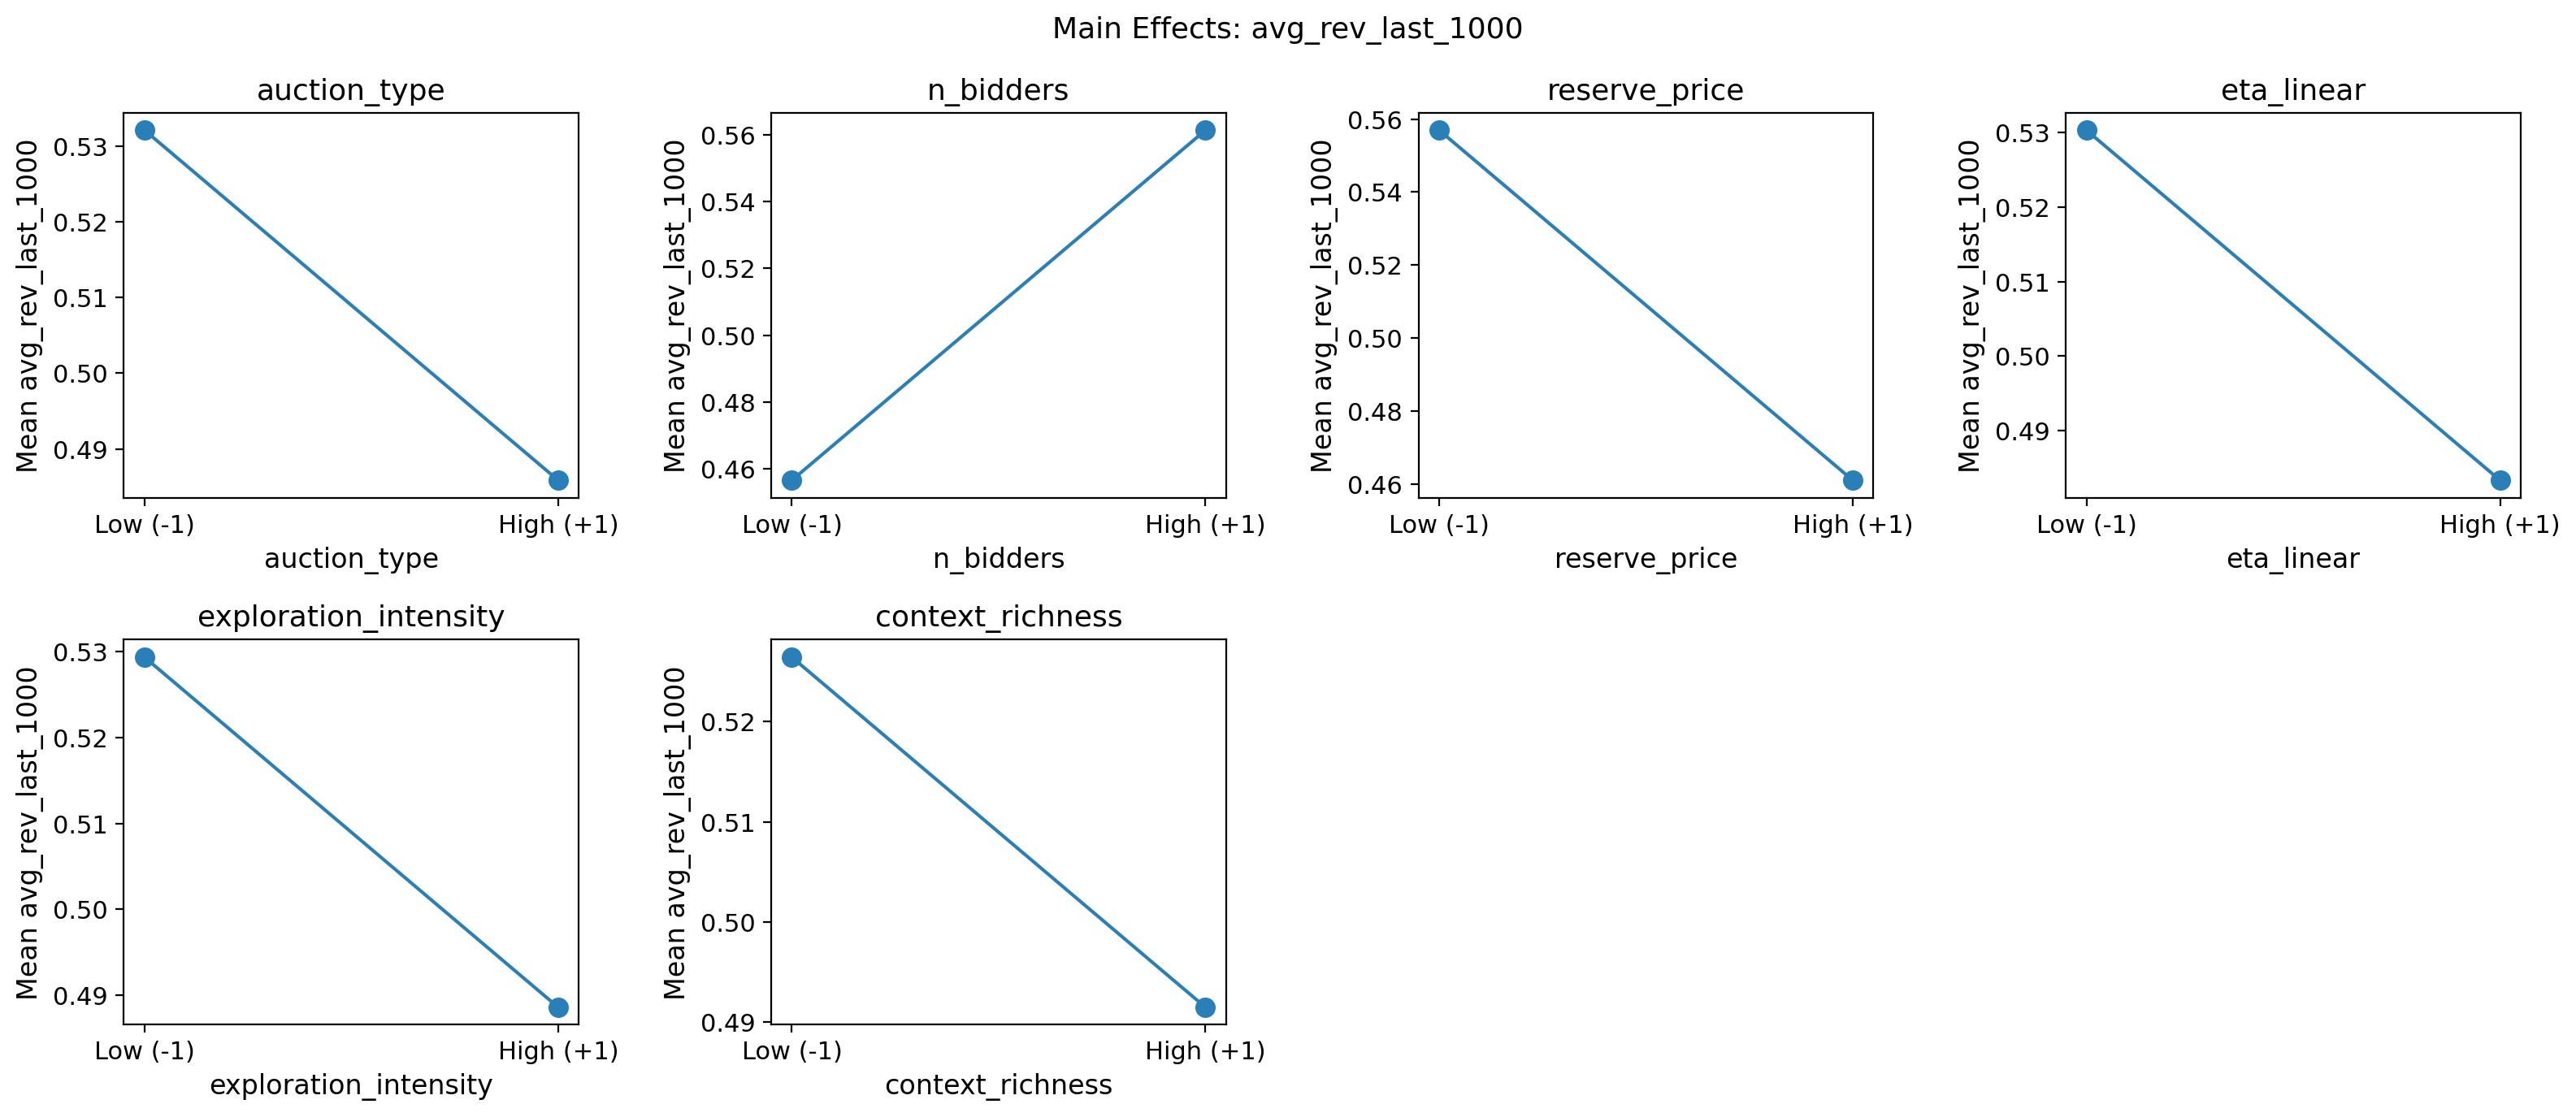
\includegraphics[width=0.7\textwidth]{figures/e2b_main_rev}
  \caption{Experiment~2b: Main effects plot for average revenue under Thompson Sampling.}
  \label{fig:e2b_main_rev}
\end{figure}

\begin{figure}[H]
  \centering
  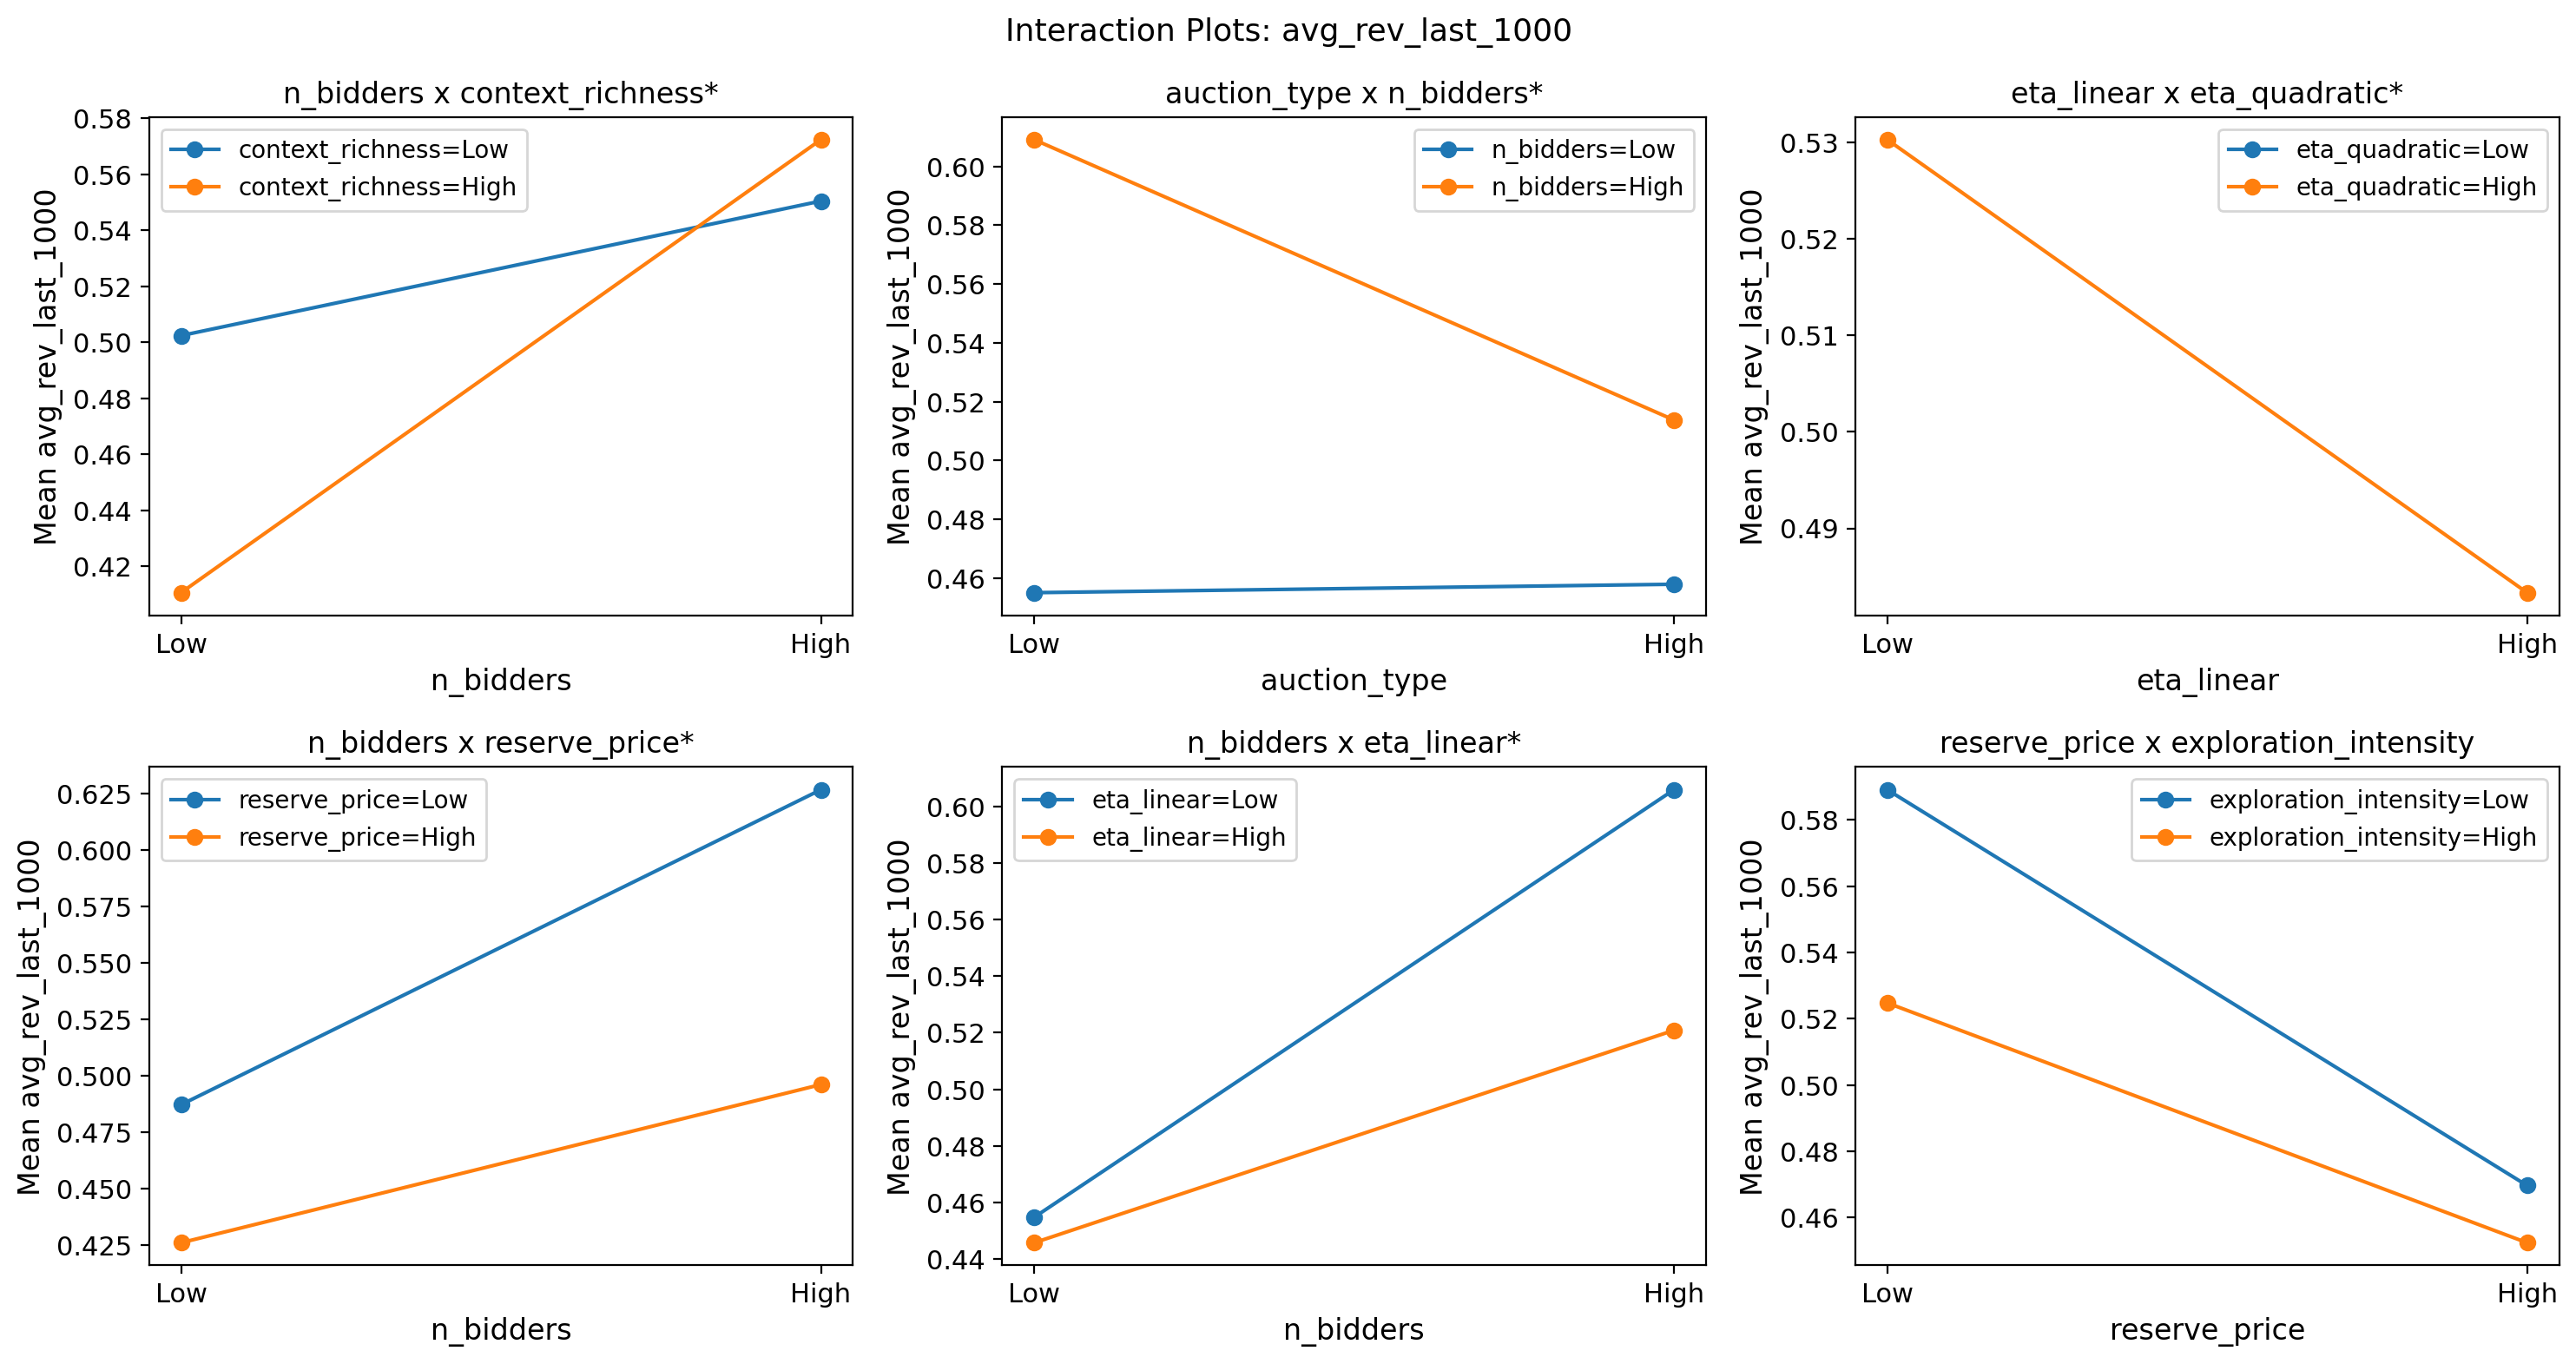
\includegraphics[width=0.7\textwidth]{figures/e2b_int_rev}
  \caption{Experiment~2b: Interaction plot for average revenue under Thompson Sampling.}
  \label{fig:e2b_int_rev}
\end{figure}

\subsubsection{Price Volatility}

Table~\ref{tab:exp2b_ranked_vol} and the main effects plot (Figure~\ref{fig:e2b_main_vol}) show the factor rankings for price volatility under Thompson Sampling.

\begin{table}[H]
\centering
\caption{Experiment 2b: Significant effects for price volatility ($p < 0.05$), ranked by $|t|$.}
\label{tab:exp2b_ranked_vol}
\begin{tabular}{lrrl}
\toprule
\textbf{Effect} & \textbf{Coeff.} & \textbf{$|t|$} & \textbf{Direction} \\
\midrule
Auction format $\times$ Number of bidders & 0.0192 & 6.57 & + \\
Number of bidders $\times$ Reserve price & 0.0180 & 6.16 & + \\
Number of bidders & -0.0177 & 6.04 & $-$ \\
Number of bidders $\times$ Context richness & -0.0156 & 5.33 & $-$ \\
Auction format & -0.0124 & 4.24 & $-$ \\
Exploration intensity & 0.0119 & 4.06 & + \\
Reserve price & 0.0106 & 3.62 & + \\
Auction format $\times$ Context richness & -0.0077 & 2.63 & $-$ \\
Reserve price $\times$ Context richness & -0.0072 & 2.45 & $-$ \\
Affiliation (linear) $\times$ Context richness & 0.0081 & 2.27 & + \\
\bottomrule
\end{tabular}
\end{table}


\begin{figure}[H]
  \centering
  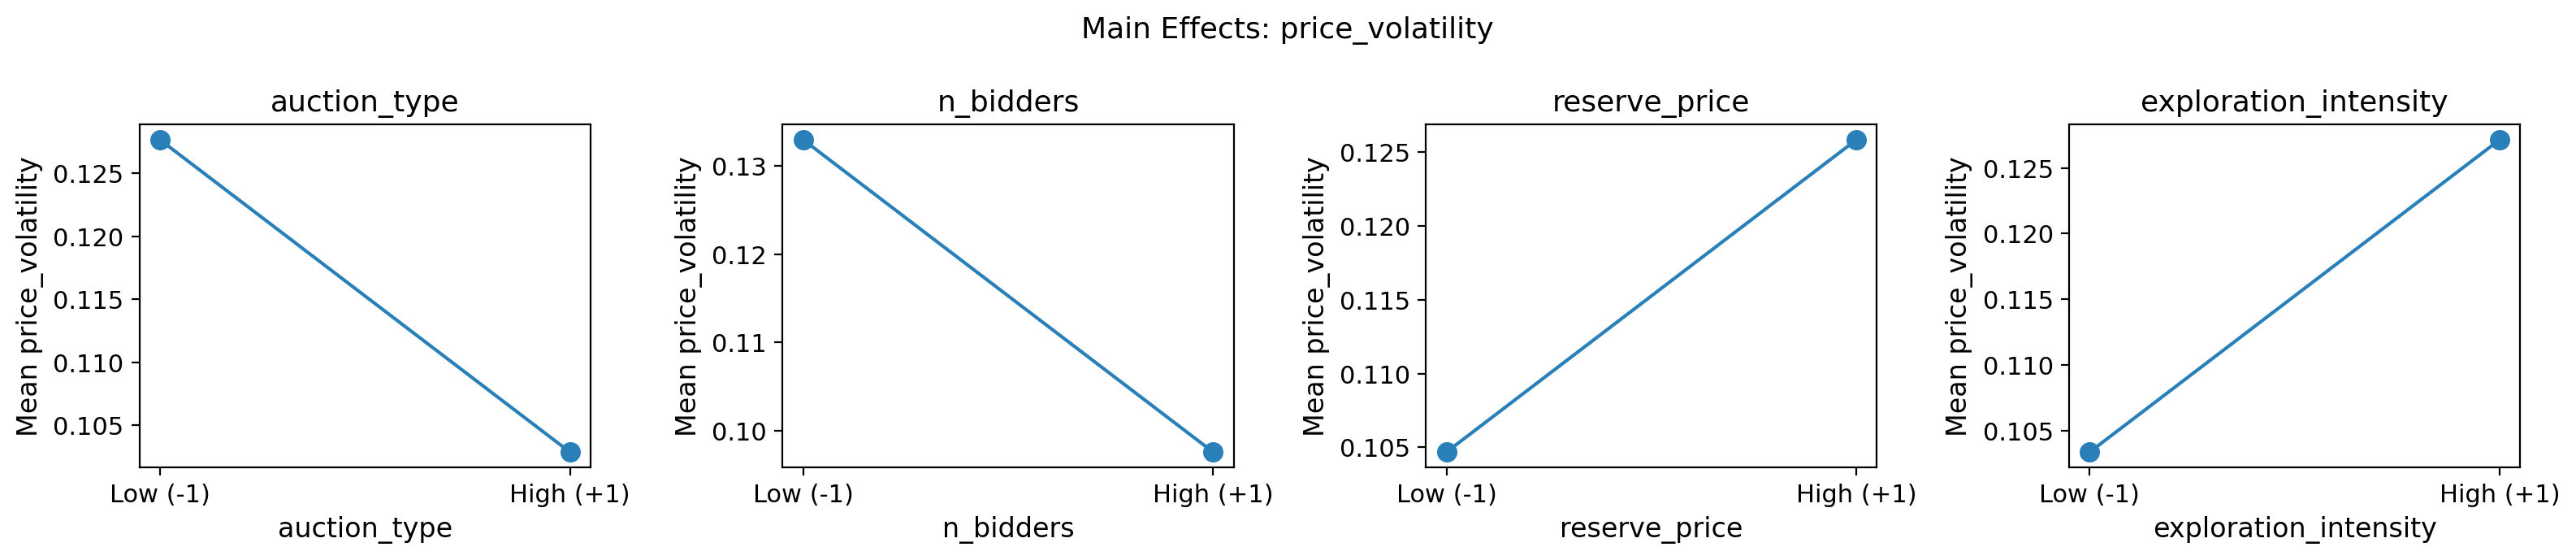
\includegraphics[width=0.7\textwidth]{figures/e2b_main_vol}
  \caption{Experiment~2b: Main effects plot for price volatility under Thompson Sampling.}
  \label{fig:e2b_main_vol}
\end{figure}

Model adequacy diagnostics confirm these findings (Appendix~\ref{sec:appendix_robustness}).

\subsection{Sensitivity Analysis}

Global sensitivity analysis confirms the factorial rankings. Under LinUCB, the number of bidders dominates four of five responses, explaining approximately half of revenue variance ($S_T = 0.55$) and nearly all winner entropy variance ($S_T = 0.75$). Algorithmic parameters (regularisation, memory decay, exploration intensity) are consistently negligible ($S_T < 0.04$). Cross-method concordance is moderate ($\rho = 0.33$). Under Thompson Sampling, factor importance is more diffuse, with no single factor exceeding $S_T = 0.31$ for revenue. Convergence time is the most diffusely driven response, with five of six factors exceeding $S_T = 0.10$. Cross-method concordance is notably low ($\rho = 0.04$), reflecting disagreement when many factors have similar importance. Detailed per-factor Sobol' indices appear in Appendix~\ref{sec:appendix_sensitivity_tables} (Tables~\ref{tab:sens_exp2a}--\ref{tab:sens_exp2b}).

\subsection{Summary}

Replacing Q-learning with contextual bandits does not improve seller welfare. Richer algorithm design does not translate into higher revenue for the auctioneer. LinUCB and Thompson Sampling respond to different design levers, validating the decision to analyse them separately. Higher exploration intensity reduces revenue under both algorithms, but the magnitudes and moderating factors differ. Global sensitivity analysis confirms these hierarchies (Appendix~\ref{sec:appendix_sensitivity_tables}). Across both algorithms, tuning parameters are consistently negligible ($S_T < 0.04$ for revenue), reinforcing the conclusion that market structure dominates algorithm configuration. Robustness checks confirm these findings (Appendix~\ref{sec:appendix_robustness}). Experiments~1a--2b share a common feature, namely that agents bid directly from value estimates without external constraints. The next section tests whether the patterns documented above persist when agents face budget constraints, the dominant paradigm in modern advertising exchanges.
